\chapter{第二格}
\begin{figure}[H]
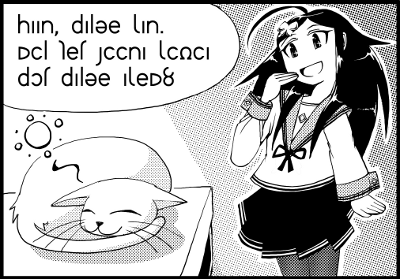
\includegraphics[width=0.5\textwidth]{ARKA/uni2.png}%或者height=\textheight
\end{figure}



\emoji{l_sena} 
那个黑发女生就是``稳重的yuule.''

她是从远方的Lutia来的.

人们说Lutia人都非常聪明,并且她,yuule尤其聪明,简直是天才.

不过有些冒失,xia她们经常调戏她.和feel关系不错.


\emoji{x_niit} 
看起来既聪明又听话.

还有冒失,嗯,是我了. 你看,把手搭在嘴边,感觉就很清爽.


\emoji{l_niit} 
嗯,除去稳重和清爽确实很像.


\emoji{x_jo} 
......

OK,我们来转写字母吧.

\FiveStar 转写

yuule: haan, palue xan. mil ket siina xidia pot palue axem?


\emoji{a_sm} 
有一些在第一格里就有了.


\emoji{x_pil} 
确实,读起来比前面更简单了.

``haan''是个感叹词,意思是``我明白了.''

还有``xan...''

我要找哪个?

----

xan

[名词]真,真实,真相

[形容词]真

[文首纯词]其实

[副词]真的,确实

[同义词]yuliet

[反义词]enx

13:制Arka:古Arka:xin (真) < xan (真实存在) < xal (存在)

xan(2)
[rente]xa
18:ridia

----

\emoji{l_sena} 
你找的是``xan(2).''

女生倾向于说``xan'',而不是``xa.''

``xa''在这.

----

xa

[动词]sol 在 yul (地点)存在

[文末纯词]注意到

[副词]状态动词的初始态

古Arka:xal

[语法]

xa (前缀): xagart (收费) 
mi (前缀): migart (免费) 

----

\emoji{x_loki} 
``xa''出现在句尾,所以是文末纯词,意思是``注意.''

这种想法就像日语的``あ、そうだ。今日は雑誌の発売日だった'',最后的``タ''\footnote{想想``哦,今天是发售日呀!''里面的``呀''}一样.

或者说,像``あぁ、あそこに見えるのは富士山か''中的``か''之类。
 

\emoji{a_reps} 
就是就是.

当发现了之前不知道的事情时就可以用``xa''.

    
\emoji{x_asex} 
所以,``haan, palue xan.''意思就是``我明白了,它的名字是洋洋.''

那就是说, yuule 明白了xia在第一格给猫起的名字.

\emoji{x_knoos} 
嘿,那个动词的``xa''呢, what does ``sol 在 yul (地点)存在''又是啥?


\emoji{l_sena_deyu} 
``sol''是主语,``yul'' 是宾语.``yul''在这时候就指地点.

如果你是主语,你在学校里,那就说``xion xa felka'',意思是``紫苑在学校.''


\emoji{x_loki} 
明白了,词典里还写了动词主语和宾语的类型.


\emoji{a_ku} 
那我顺便就教你动词搭配吧.关于什么样的名词和动词搭配.

``xa''的搭配,是``sol (人/物)在 yul (地点).''

每个动词都有自己的搭配:``lat (放入)''的搭配是``sol (人) 使 yul (人/物) 进入 a (地点).''

----

lat

[动词]sol (人) 使 yul (人/物) 进入 a (地点)

[名词]入口

[动词]收拾 > fitl

[动词]进入学校或公司 > lod

[antonym]rik

13:制Arka:古Arka:luta (出)

【成句】

hino yul sa lat 差一点就/到极限了

lat, toot, zok, rik 起承转合。入口、坡道、顶上、出口:比喻山路。

【用例】
an hinot ena sa lat. 努力忍住眼泪。

an hinot jo sa lat. 差点就爆发了。
----

\emoji{x_niit} 
你看下动词搭配,就知道该用哪些词了.


\emoji{l_diina} 
下一句是``mil ket siina xidia pot palue axem?''.

我给你解释下``mil''字典说它表示较弱的推断.

``因为''是``man'',这在Lein课1里面讲过了.但是 ``mil''也是 ``因为.''


\emoji{x_knoos} 
那他俩有什么区别呢?


\emoji{l_deyu} 
``man''表示原因和结果的距离近. ``mil''则表示原因较弱,我的意思是,不稳定.

女生倾向用``mil'',少用``man'',这是为了舒缓语气.


\emoji{x_asex} 
OK, ``mil'' 表示 ``因为'',句子是 ``mil ket siina xidia pot palue axem?.''

``ket''是主语``猫'',``siina''是动词``喜欢.''

``xidia''是 ``梦.'' 那么句子的意思是 ``猫喜欢梦.''?


\emoji{l_reia} 
不是,``xidia''也是动词.句子里有两个动词.

``xidia''确实是 ``梦,''不过这里只表示 ``睡觉'' ,这是女生的委婉哦.本来``睡觉''是``mok''.


\emoji{x_loki} 
所以这个句子的意思是``Cats like to sleep.''

那 ``pot''又是什么意思?

----

pot

[名词]内部

[格词]在...里面

[反义词]tant

古Arka:pot, poto

----

\emoji{x_lo} 
``pot''是一个介词,意思是``in.''

``pot palue''意思是 ``在palue里面.''

不过,palue不是那只猫的名字吗. ``他喜欢睡在他里面''?!


\emoji{a_naki} 
啊,不不,不是, ``pot palue'' 里面的palue是个名词,表示``有太阳的地方.''

他的名字也表示``有太阳的地方''.


\emoji{x_asex} 
现在我明白了.

``mil ket siina xidia pot palue axem?''意思是``猫喜欢睡在有太阳的地方,所以你叫它洋洋,对吧?''

yuule这是在确认她的想法.


\emoji{l_ket} 
对.

你已经到漫画的折返点了. atte! (加油!)











